\chapter[Maxent]{Máxima Entropia}

\begin{objetivos}
	Ao final desta unidade, o estudante deverá compreender os fundamentos do Maxent em SDM; interpretar o princípio da máxima entropia; diferenciar features lineares, quadráticas, hinge e produto; compreender o papel da regularização; ajustar modelos Maxent com dados presença-background de \textit{Dinizia excelsa}; realizar tuning de feature classes e regularization multiplier; avaliar o modelo com AUC, TSS, sensibilidade e especificidade; gerar curvas de resposta; produzir mapa de adequabilidade ambiental atual; e comparar Maxent com GLM, GAM, Random Forest e BRT.
\end{objetivos}

\section{Introdução}

O Maxent é um dos métodos mais utilizados em Modelagem de Distribuição de Espécies, especialmente quando os dados disponíveis são registros de presença e pontos de background. O método estima uma distribuição de máxima entropia, isto é, a distribuição mais uniforme possível, sujeita às restrições impostas pelas condições ambientais observadas nos locais de presença \parencite{phillips2006maximum,phillips2008modeling,elith2011statistical,merow2013practical,guisan2017habitat}.

Em termos práticos, o Maxent compara os valores ambientais nas presenças com os valores ambientais disponíveis no background. A partir dessa comparação, estima uma função de adequabilidade relativa que indica quais combinações ambientais são mais semelhantes às condições onde a espécie foi observada.

\begin{conceito}[title={\faBook\quad Maxent em SDM}]
	Maxent é um método presença-background baseado no princípio da máxima entropia. Ele estima uma distribuição espacial de adequabilidade ambiental que satisfaz as restrições ambientais observadas nas presenças, evitando assumir mais estrutura do que a informação disponível permite.
\end{conceito}

\section{Máxima entropia e adequabilidade ambiental}

O princípio da máxima entropia busca a distribuição menos enviesada possível, dado um conjunto de restrições. Em SDM, essas restrições são derivadas das variáveis ambientais nos pontos de presença. Assim, o modelo busca uma distribuição que seja o mais uniforme possível, mas que respeite as características ambientais associadas à ocorrência da espécie.

\begin{equationbox}
	\[
	\hat{p}(x) =
	\frac{\exp\left(\sum_j \lambda_j f_j(x)\right)}
	{Z}
	\]
\end{equationbox}

em que \(\hat{p}(x)\) representa a adequabilidade relativa em um local \(x\), \(f_j(x)\) são funções das variáveis ambientais, \(\lambda_j\) são pesos estimados pelo modelo e \(Z\) é uma constante de normalização.

\section{Feature classes}

No Maxent, as relações entre espécie e ambiente são representadas por diferentes tipos de funções, chamadas \textit{feature classes}. As principais são:

\begin{itemize}
	\item linear (L): respostas lineares;
	\item quadratic (Q): respostas unimodais ou em forma de parábola;
	\item product (P): interações entre variáveis;
	\item hinge (H): respostas com limiares e mudanças abruptas;
	\item threshold (T): respostas por cortes discretos.
\end{itemize}

\begin{atencao}[title={\faExclamationTriangle\quad Complexidade do Maxent}]
	Modelos Maxent com muitas features e baixa regularização podem apresentar sobreajuste. Por isso, a escolha de feature classes e do parâmetro de regularização deve ser feita por tuning e validação independente.
\end{atencao}

\section{Regularização}

A regularização controla a complexidade do modelo. Valores baixos permitem respostas mais flexíveis, mas aumentam o risco de sobreajuste. Valores altos tornam o modelo mais simples e suave, podendo reduzir a capacidade de capturar padrões ecológicos reais. O parâmetro geralmente avaliado é o \textit{regularization multiplier}.

\begin{conceito}[title={\faBook\quad Regularização}]
	A regularização penaliza modelos excessivamente complexos. Em SDM, ela é fundamental para aumentar a capacidade de transferência espacial e temporal, especialmente em projeções futuras ou paleoclimáticas.
\end{conceito}

\section{Preparação dos dados}

Nesta unidade utilizamos a base presença-background construída na Unidade 5 e as variáveis selecionadas na Unidade 4. O ajuste será feito com o pacote \texttt{maxnet}, uma implementação em R do Maxent baseada em modelos penalizados, sem necessidade do arquivo Java \texttt{maxent.jar}.

\rscriptfile{scripts/unidade10/01_estrutura_pastas.R}

\rscriptfile{scripts/unidade10/02_preparar_dados_maxent.R}

\section{Tuning de feature classes e regularização}

O tuning avalia diferentes combinações de feature classes e multiplicadores de regularização. O objetivo é escolher um modelo com bom desempenho preditivo, mas sem complexidade excessiva.

\rscriptfile{scripts/unidade10/03_tuning_maxent_dinizia.R}

\begin{figure}[H]
	\centering
	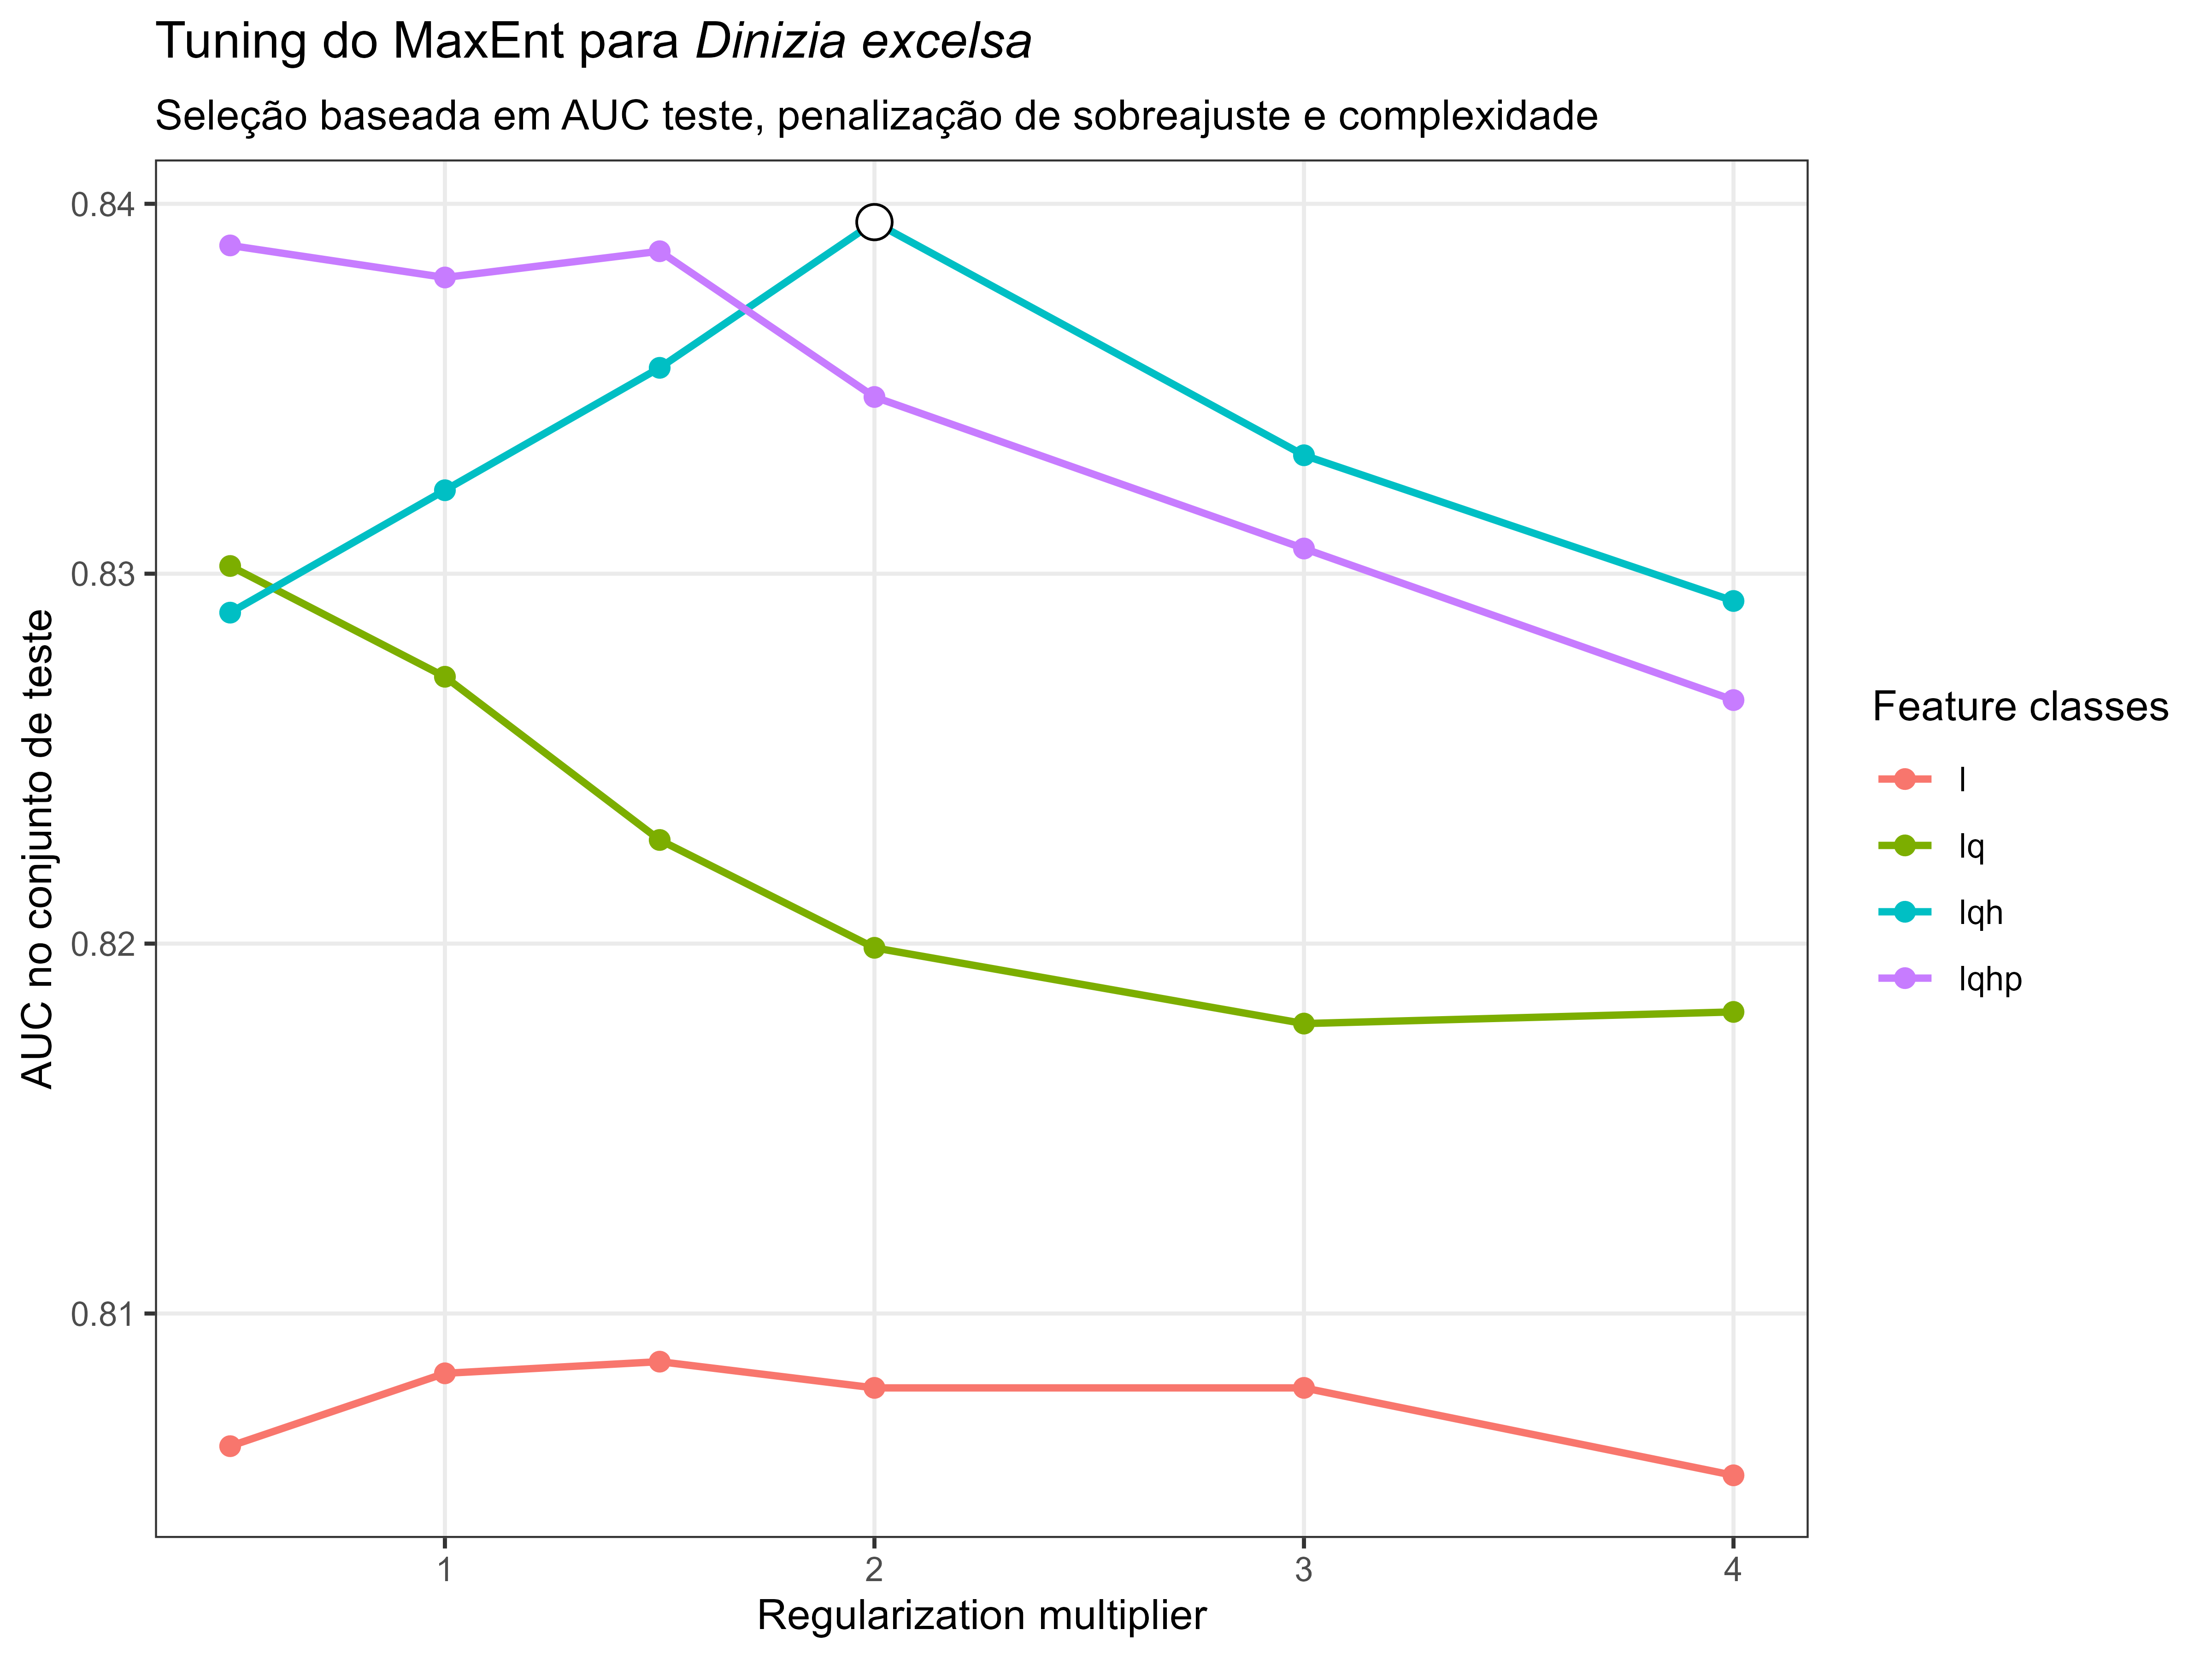
\includegraphics[width=0.88\textwidth]{figuras/unidade10/unidade10_tuning_maxent.png}
	\caption{Resultados do tuning do Maxent para \textit{Dinizia excelsa}, considerando diferentes combinações de feature classes e regularization multiplier.}
	\label{fig:unidade10_tuning_maxent}
\end{figure}

\section{Ajuste do modelo Maxent final}

Após o tuning, o melhor conjunto de hiperparâmetros é usado para ajustar o modelo final.

\rscriptfile{scripts/unidade10/04_ajustar_maxent_final.R}

\begin{figure}[H]
	\centering
	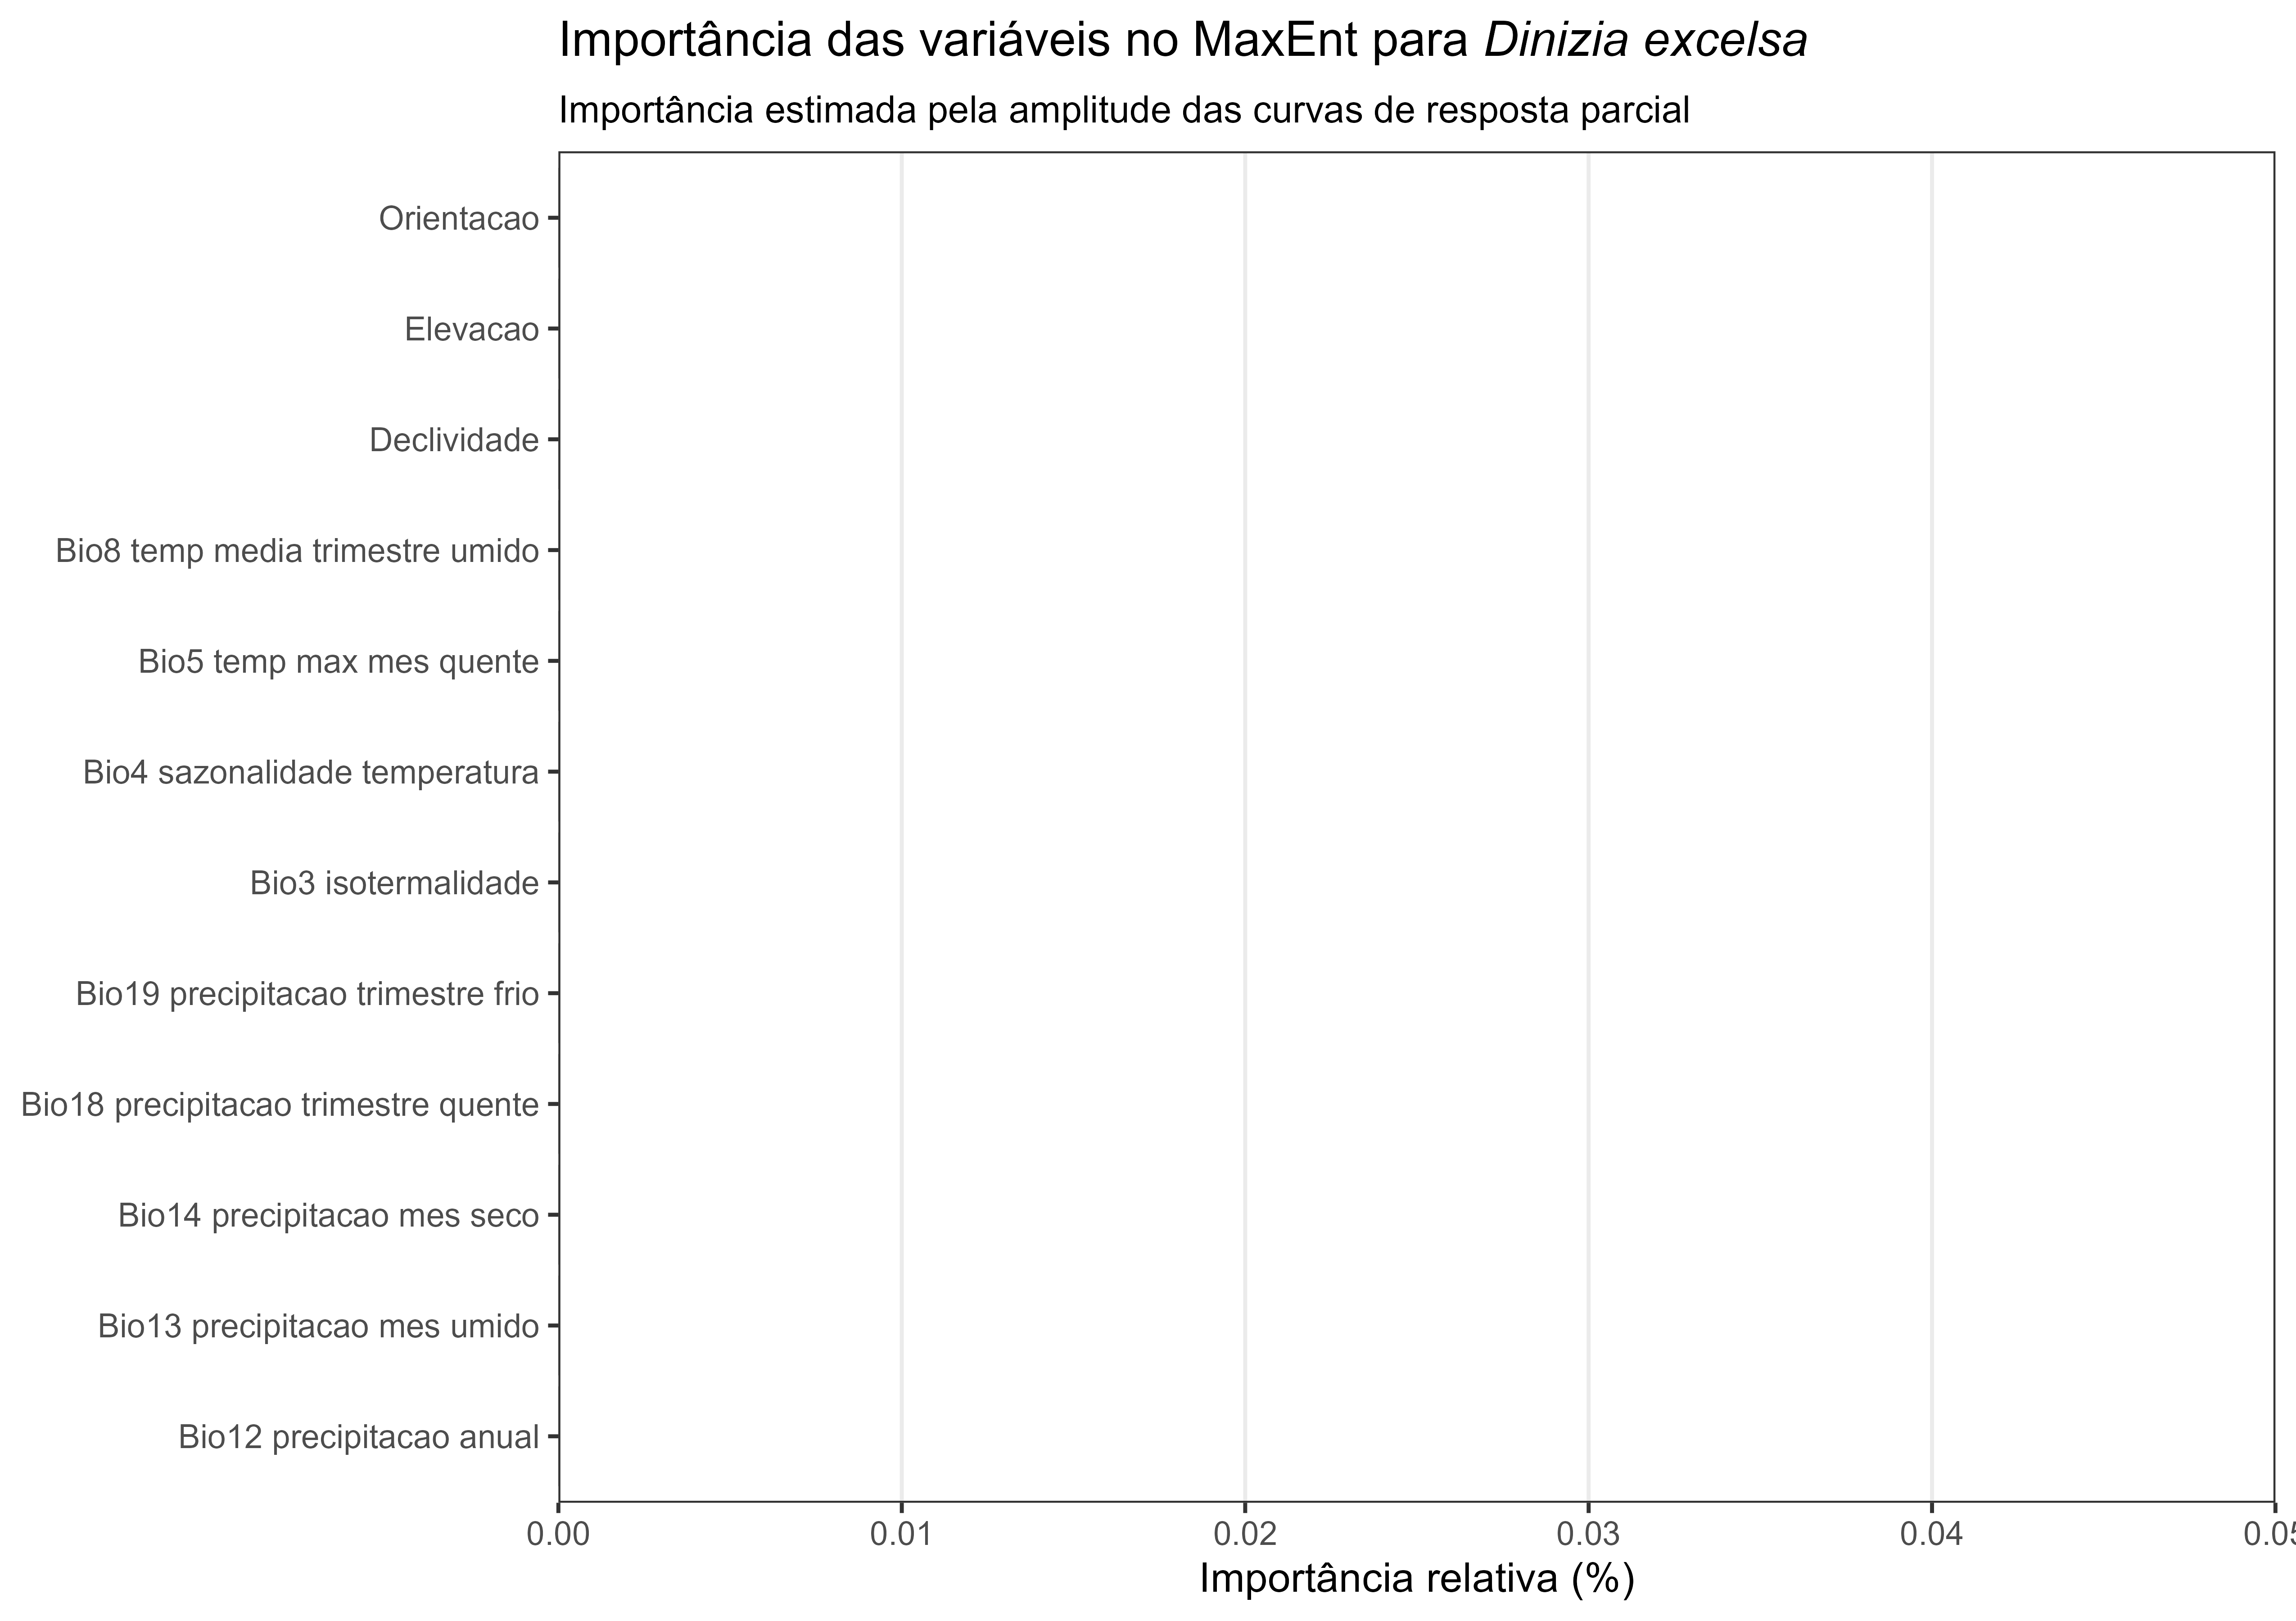
\includegraphics[width=0.86\textwidth]{figuras/unidade10/unidade10_importancia_variaveis_maxent.png}
	\caption{Importância relativa das variáveis ambientais no modelo Maxent final ajustado para \textit{Dinizia excelsa}.}
	\label{fig:unidade10_importancia_maxent}
\end{figure}

\section{Avaliação do modelo}

O modelo Maxent é avaliado com dados de teste independentes usando AUC, TSS, sensibilidade, especificidade e matriz de confusão.

\rscriptfile{scripts/unidade10/05_avaliar_maxent_dinizia.R}

\begin{figure}[H]
	\centering
	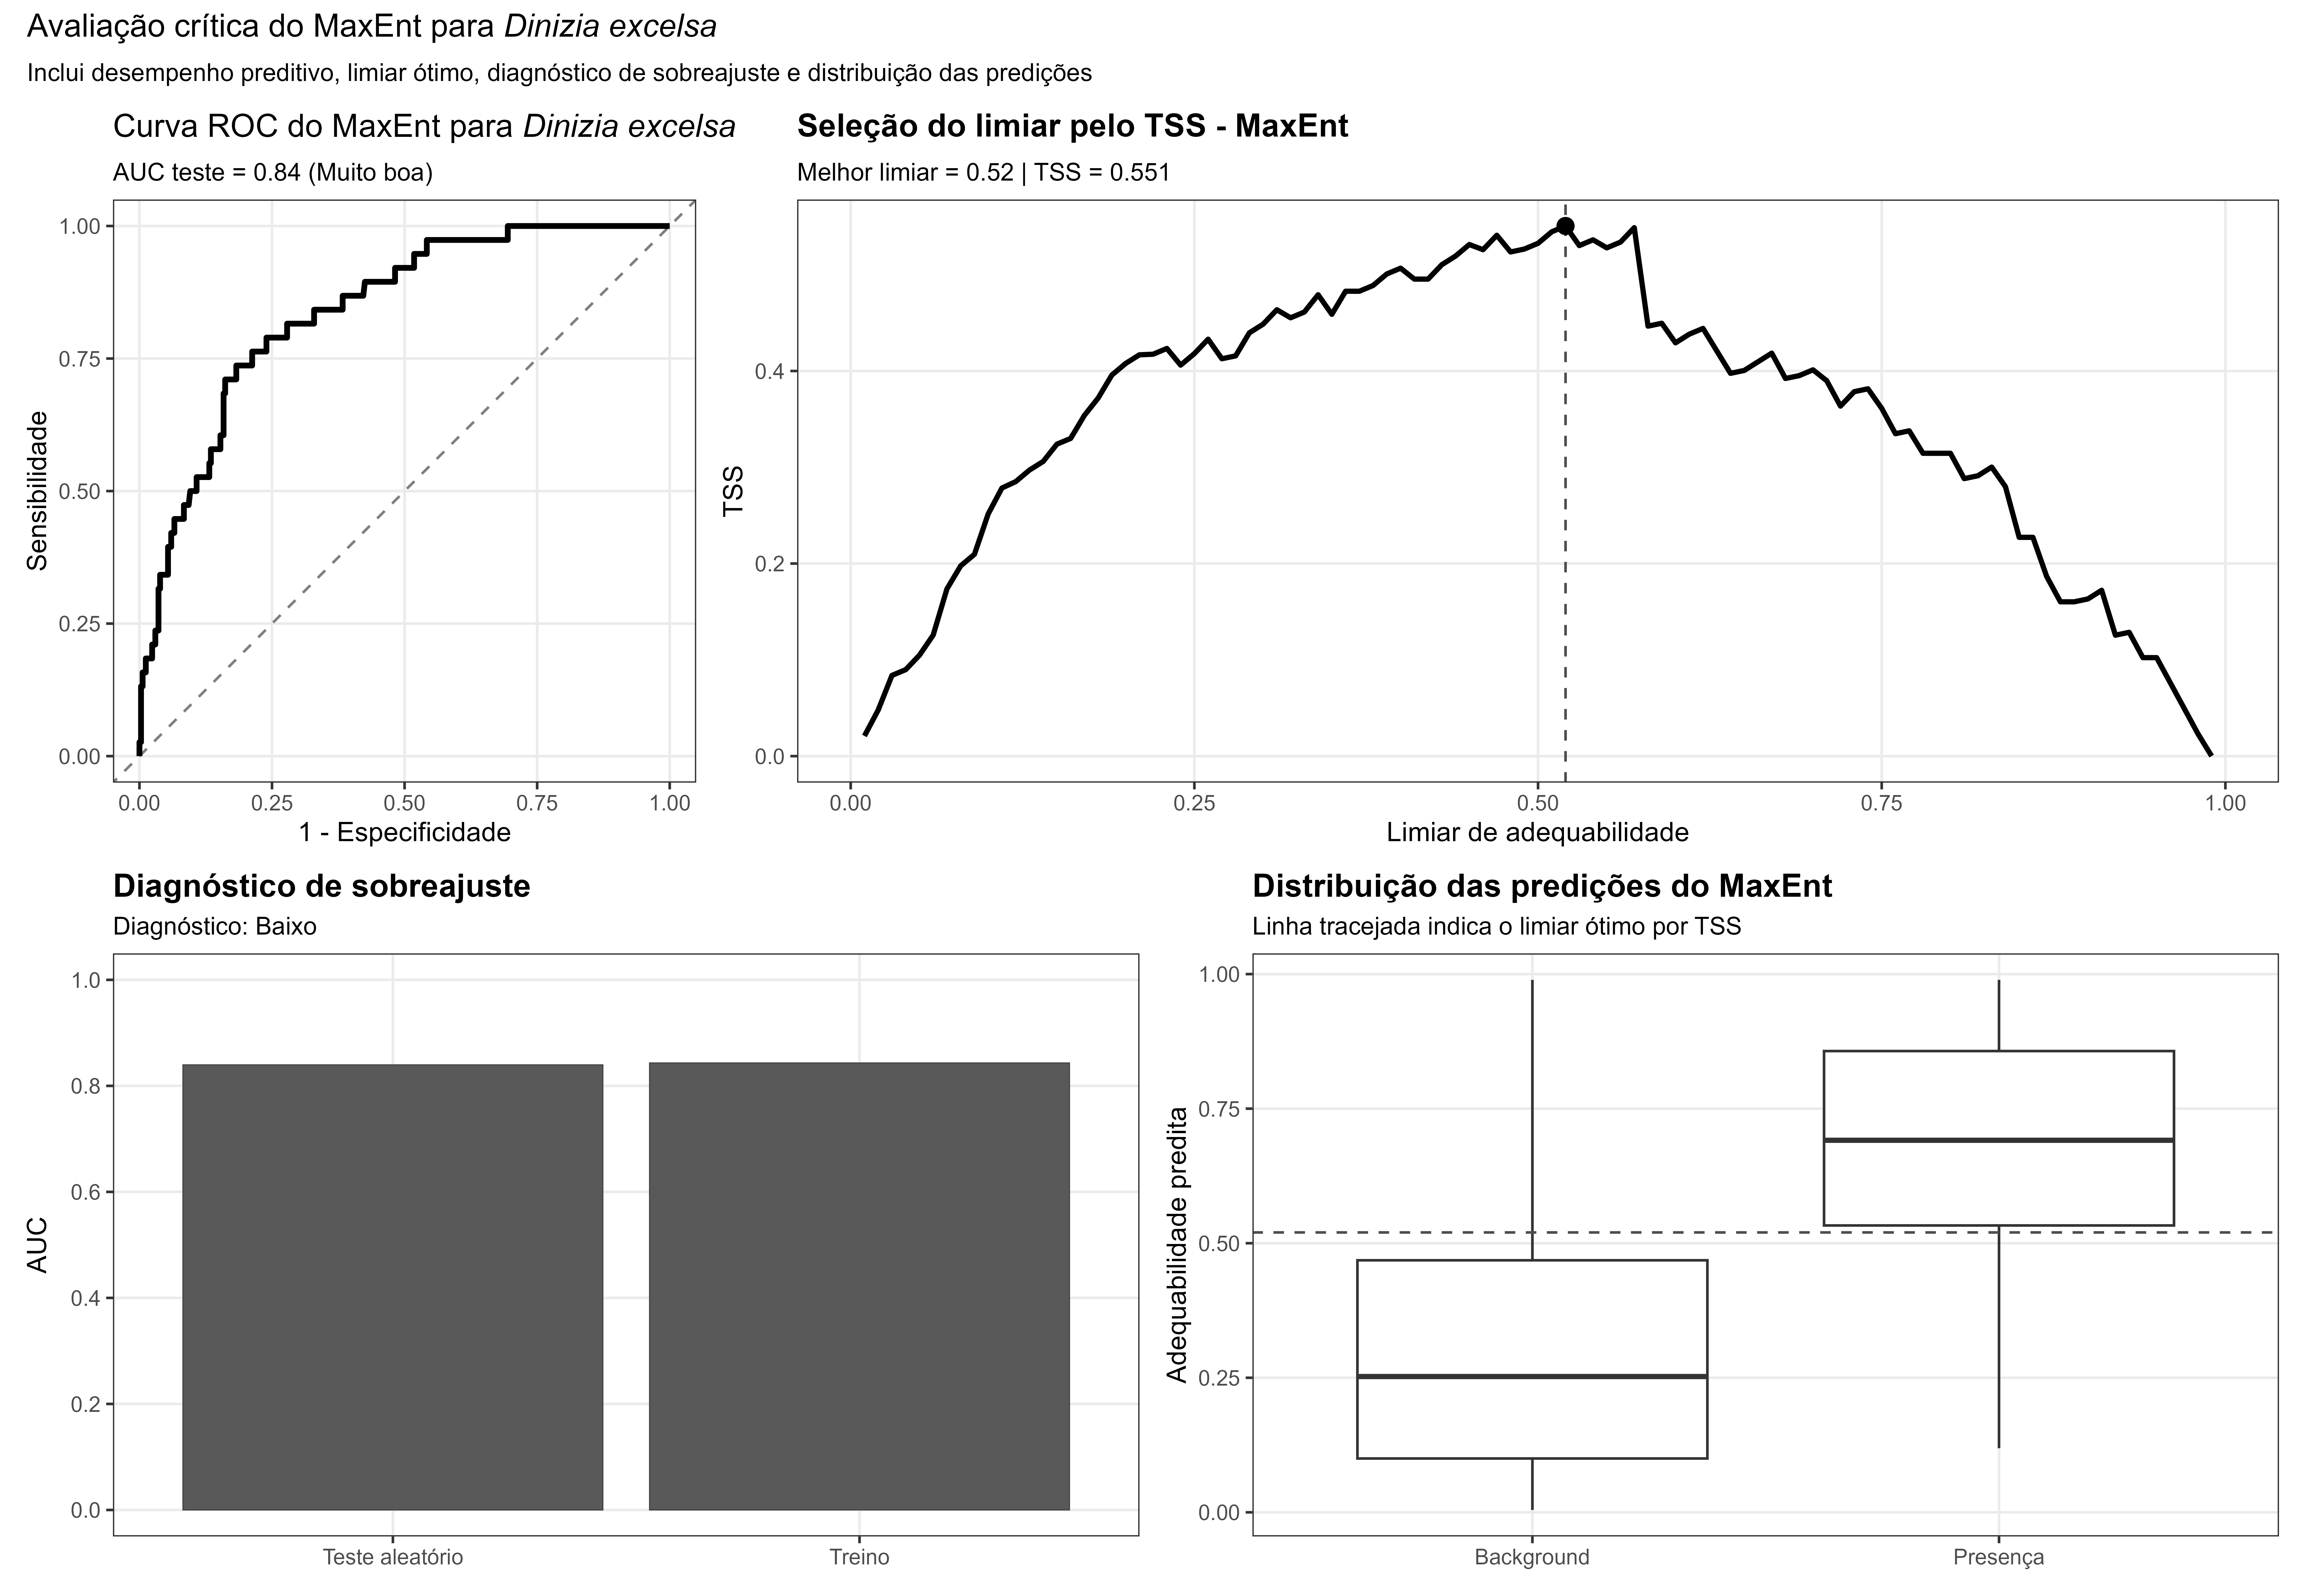
\includegraphics[width=0.78\textwidth]{figuras/unidade10/unidade10_avaliacao_maxent_patchwork.png}
	\caption{Curva ROC do Maxent avaliado no conjunto teste para \textit{Dinizia excelsa}.}
	\label{fig:unidade10_roc_maxent}
\end{figure}

\section{Mapa de adequabilidade atual}

O modelo final é projetado espacialmente para a área acessível \(M\), produzindo um mapa contínuo de adequabilidade ambiental atual.

\rscriptfile{scripts/unidade10/06_predicao_espacial_maxent.R}

\begin{figure}[H]
	\centering
	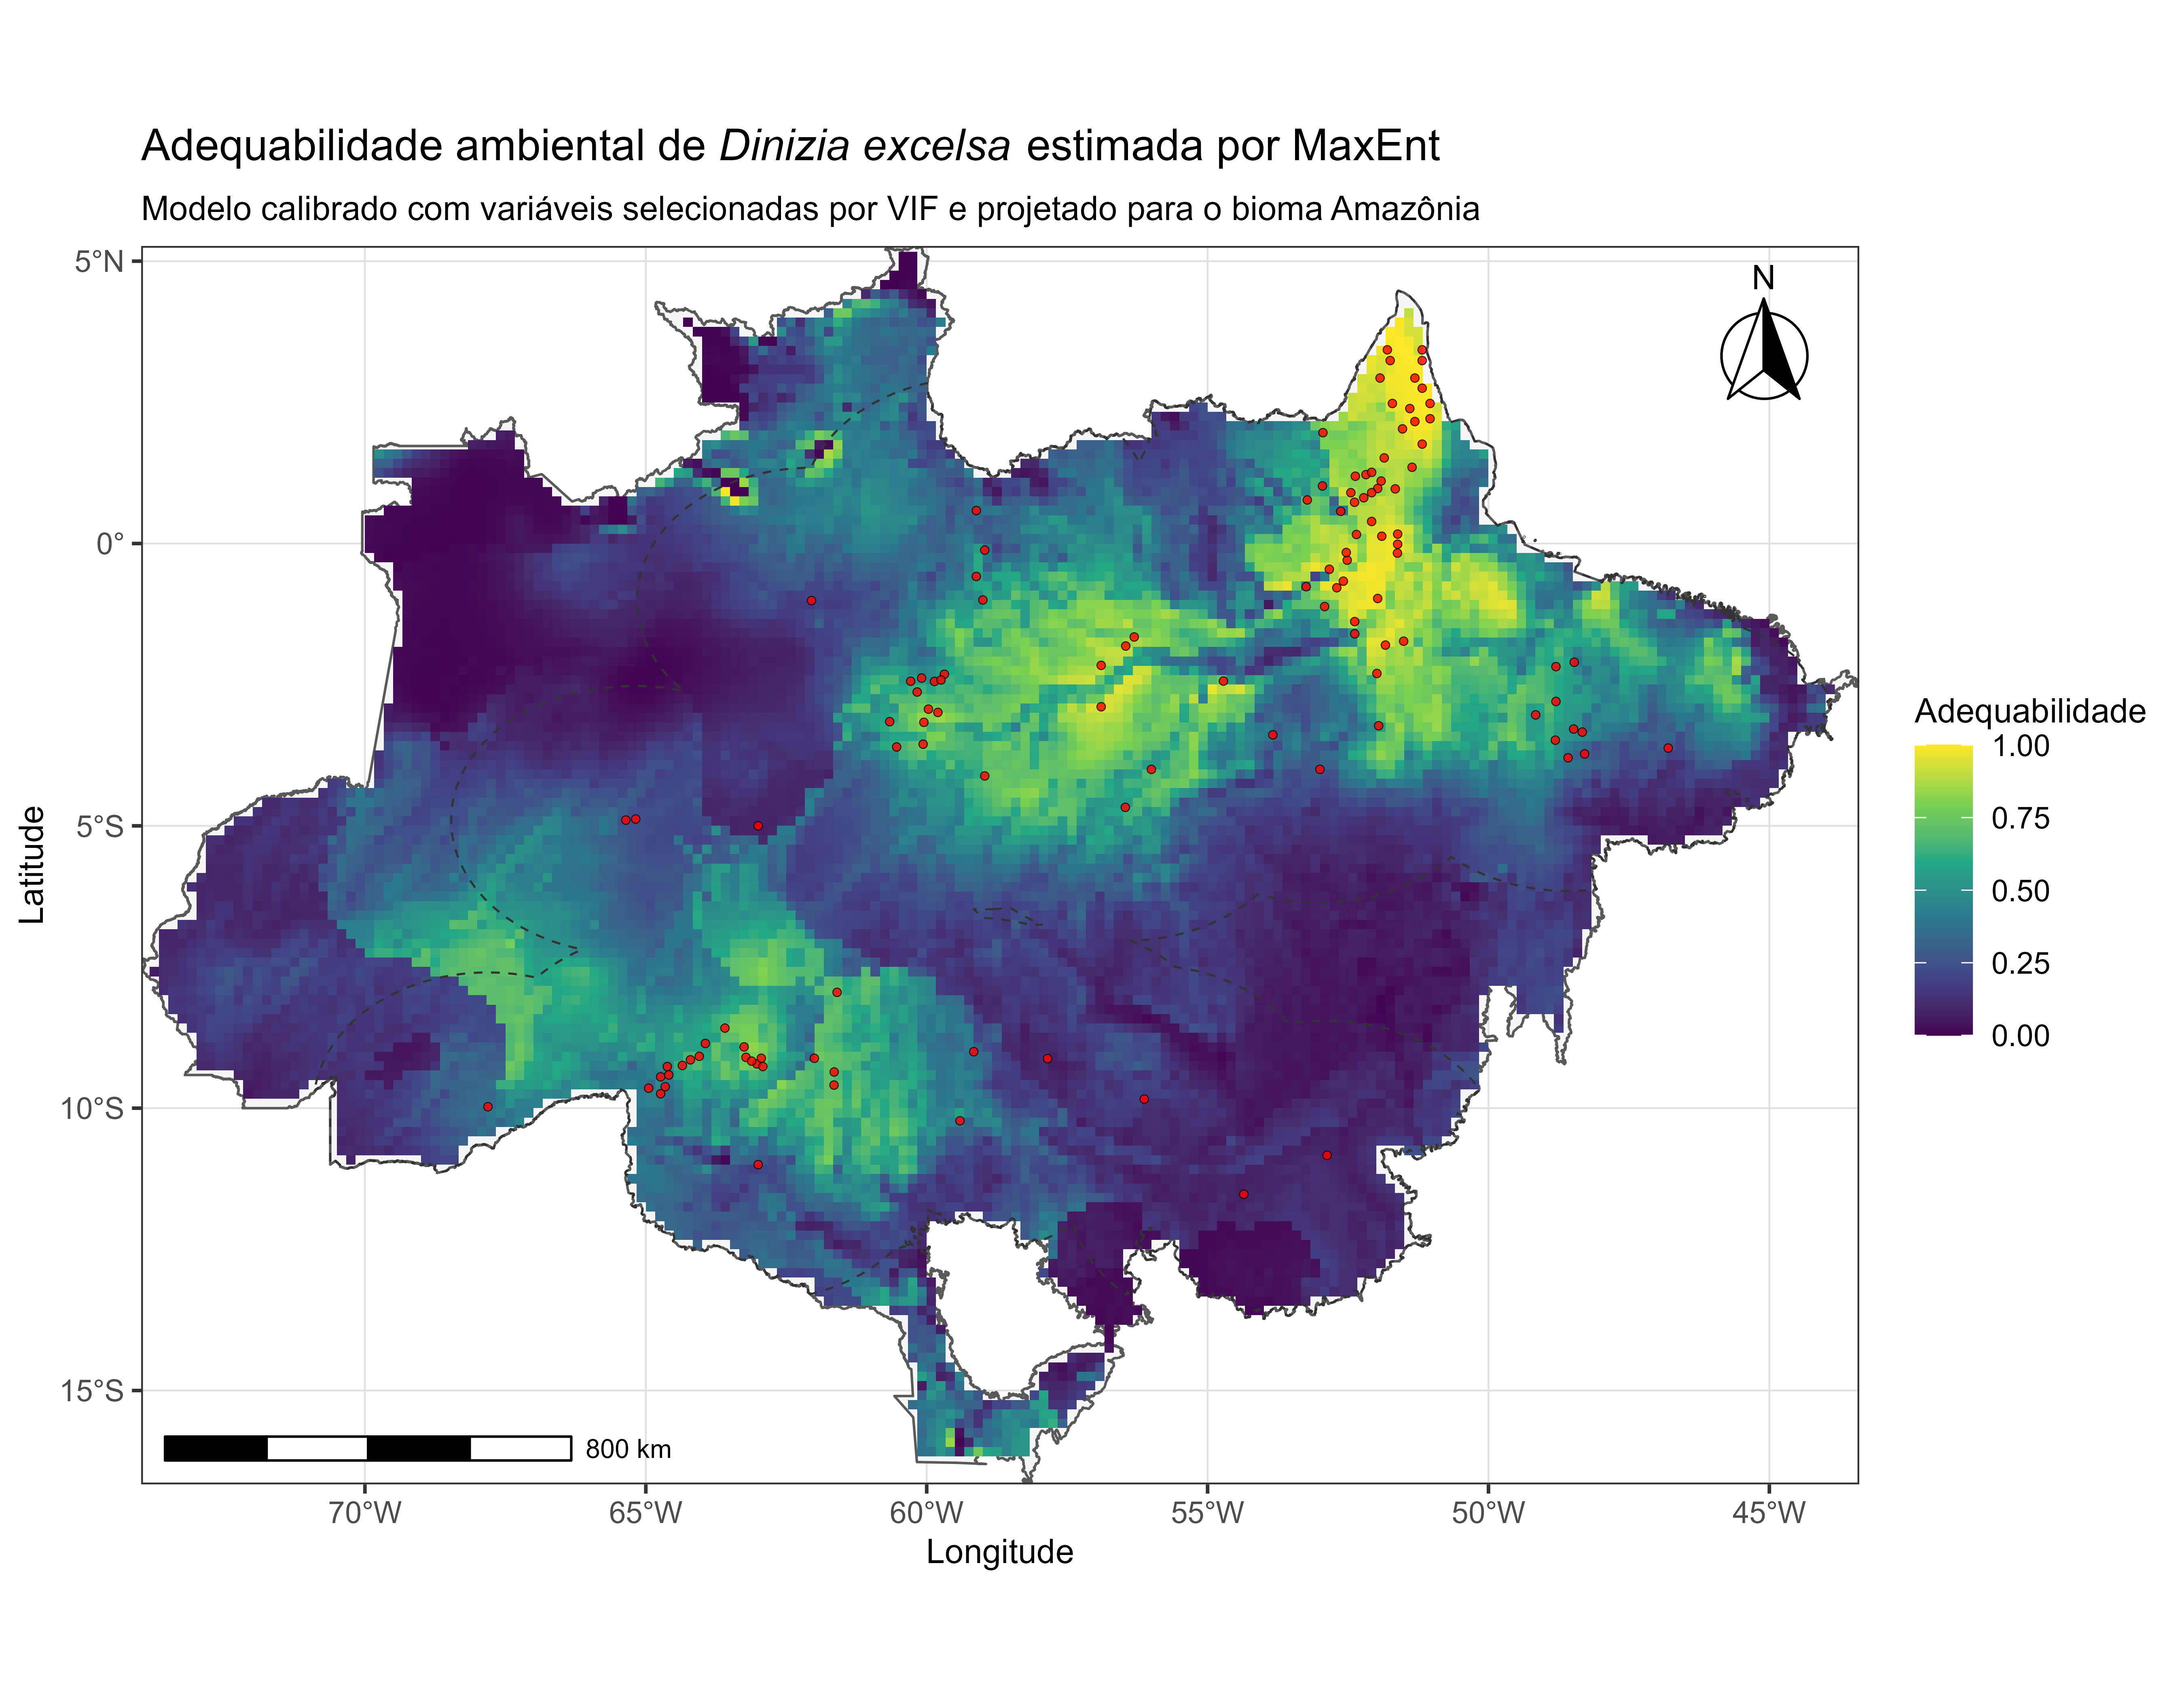
\includegraphics[width=0.88\textwidth]{figuras/unidade10/unidade10_adequabilidade_maxent.png}
	\caption{Mapa de adequabilidade ambiental atual de \textit{Dinizia excelsa} estimado por Maxent dentro da área acessível \(M\).}
	\label{fig:unidade10_adequabilidade_maxent}
\end{figure}

\section{Curvas de resposta parcial}

As curvas de resposta parcial permitem visualizar como a adequabilidade estimada pelo Maxent varia ao longo dos gradientes ambientais selecionados.

\rscriptfile{scripts/unidade10/07_curvas_resposta_maxent.R}

\begin{figure}[H]
	\centering
	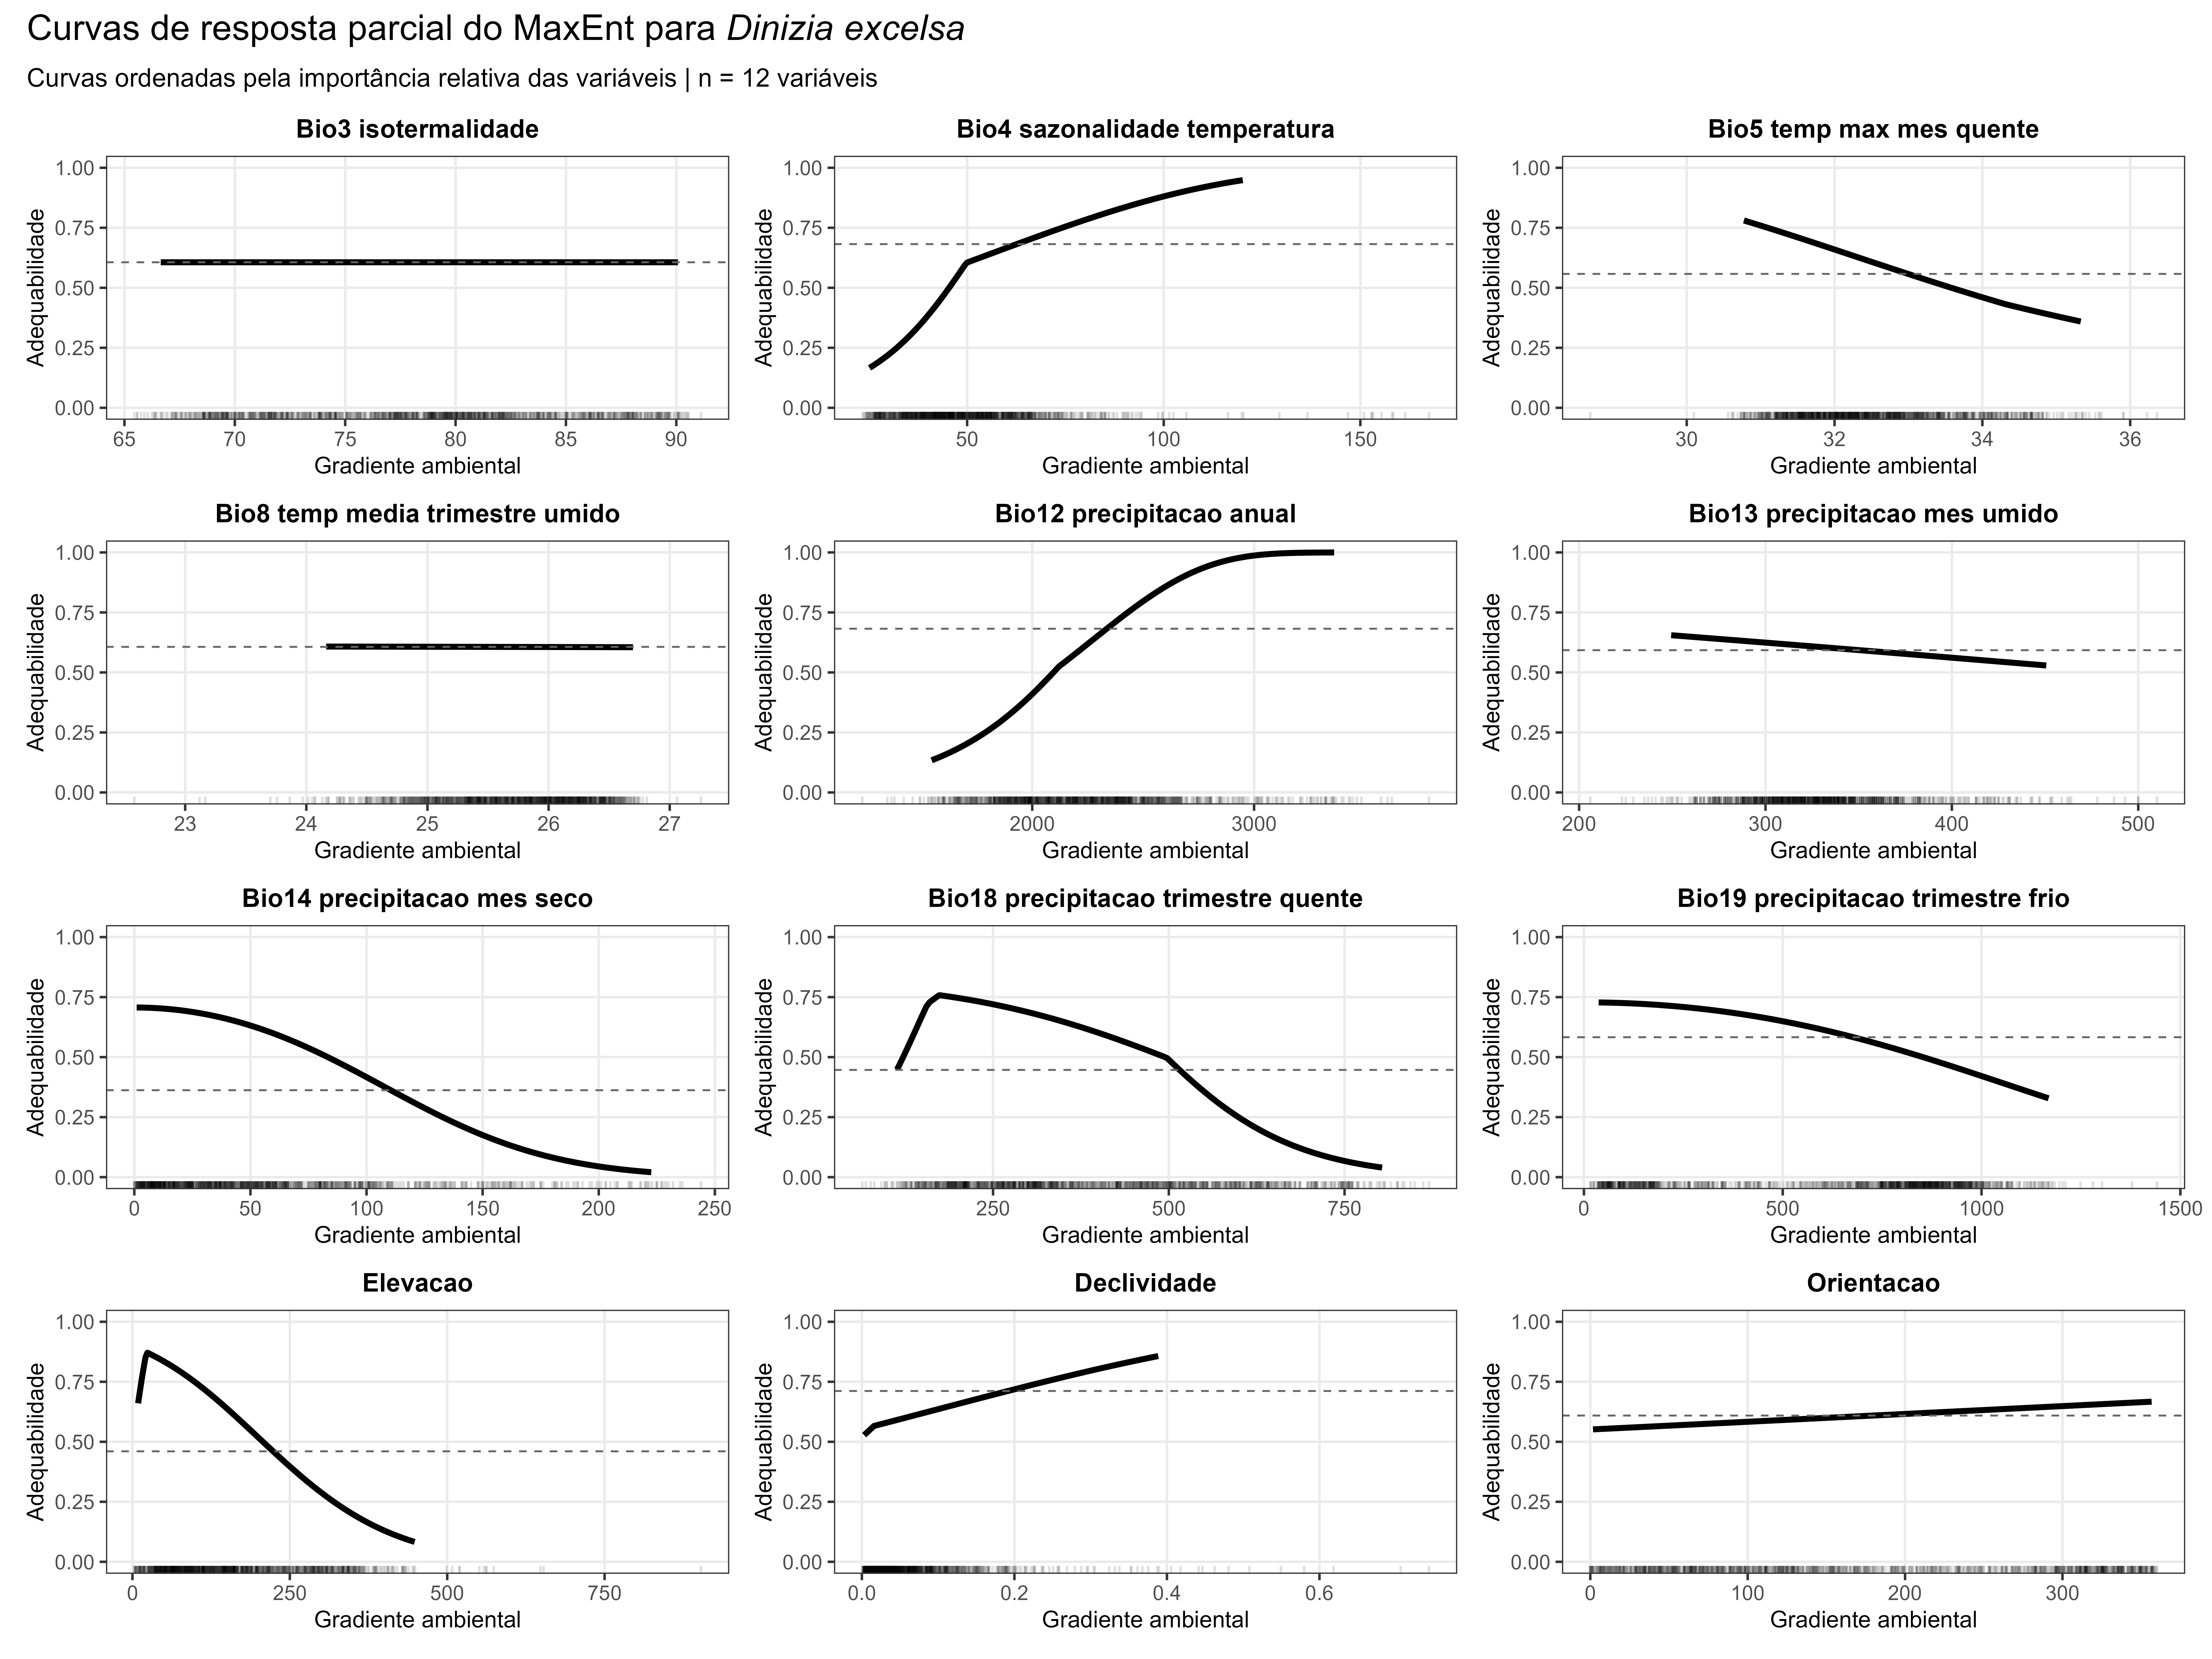
\includegraphics[width=0.96\textwidth]{figuras/unidade10/unidade10_curvas_resposta_maxent.png}
	\caption{Curvas de resposta parcial do Maxent para as variáveis ambientais selecionadas.}
	\label{fig:unidade10_curvas_resposta_maxent}
\end{figure}

\section{Comparação com os modelos anteriores}

\rscriptfile{scripts/unidade10/08_comparar_modelos_maxent.R}

\begin{figure}[H]
	\centering
	\includegraphics[width=0.98\textwidth]{figuras/unidade10/unidade10_comparacao_modelos_maxent.png}
	\caption{Comparação entre mapas de adequabilidade estimados por GLM, GAM, Random Forest, BRT e Maxent.}
	\label{fig:unidade10_comparacao_modelos}
\end{figure}

\section{Pipeline completo}

\rscriptfile{scripts/unidade10/09_pipeline_maxent.R}

\section{Síntese da unidade}

O Maxent é um método robusto, amplamente utilizado e especialmente adequado para dados de presença-background. Entretanto, sua aplicação exige decisões cuidadosas sobre background, feature classes, regularização, tuning e validação. Modelos excessivamente complexos podem produzir mapas aparentemente detalhados, mas pouco transferíveis para outros períodos climáticos ou regiões.

\begin{figure}[H]
	\centering
	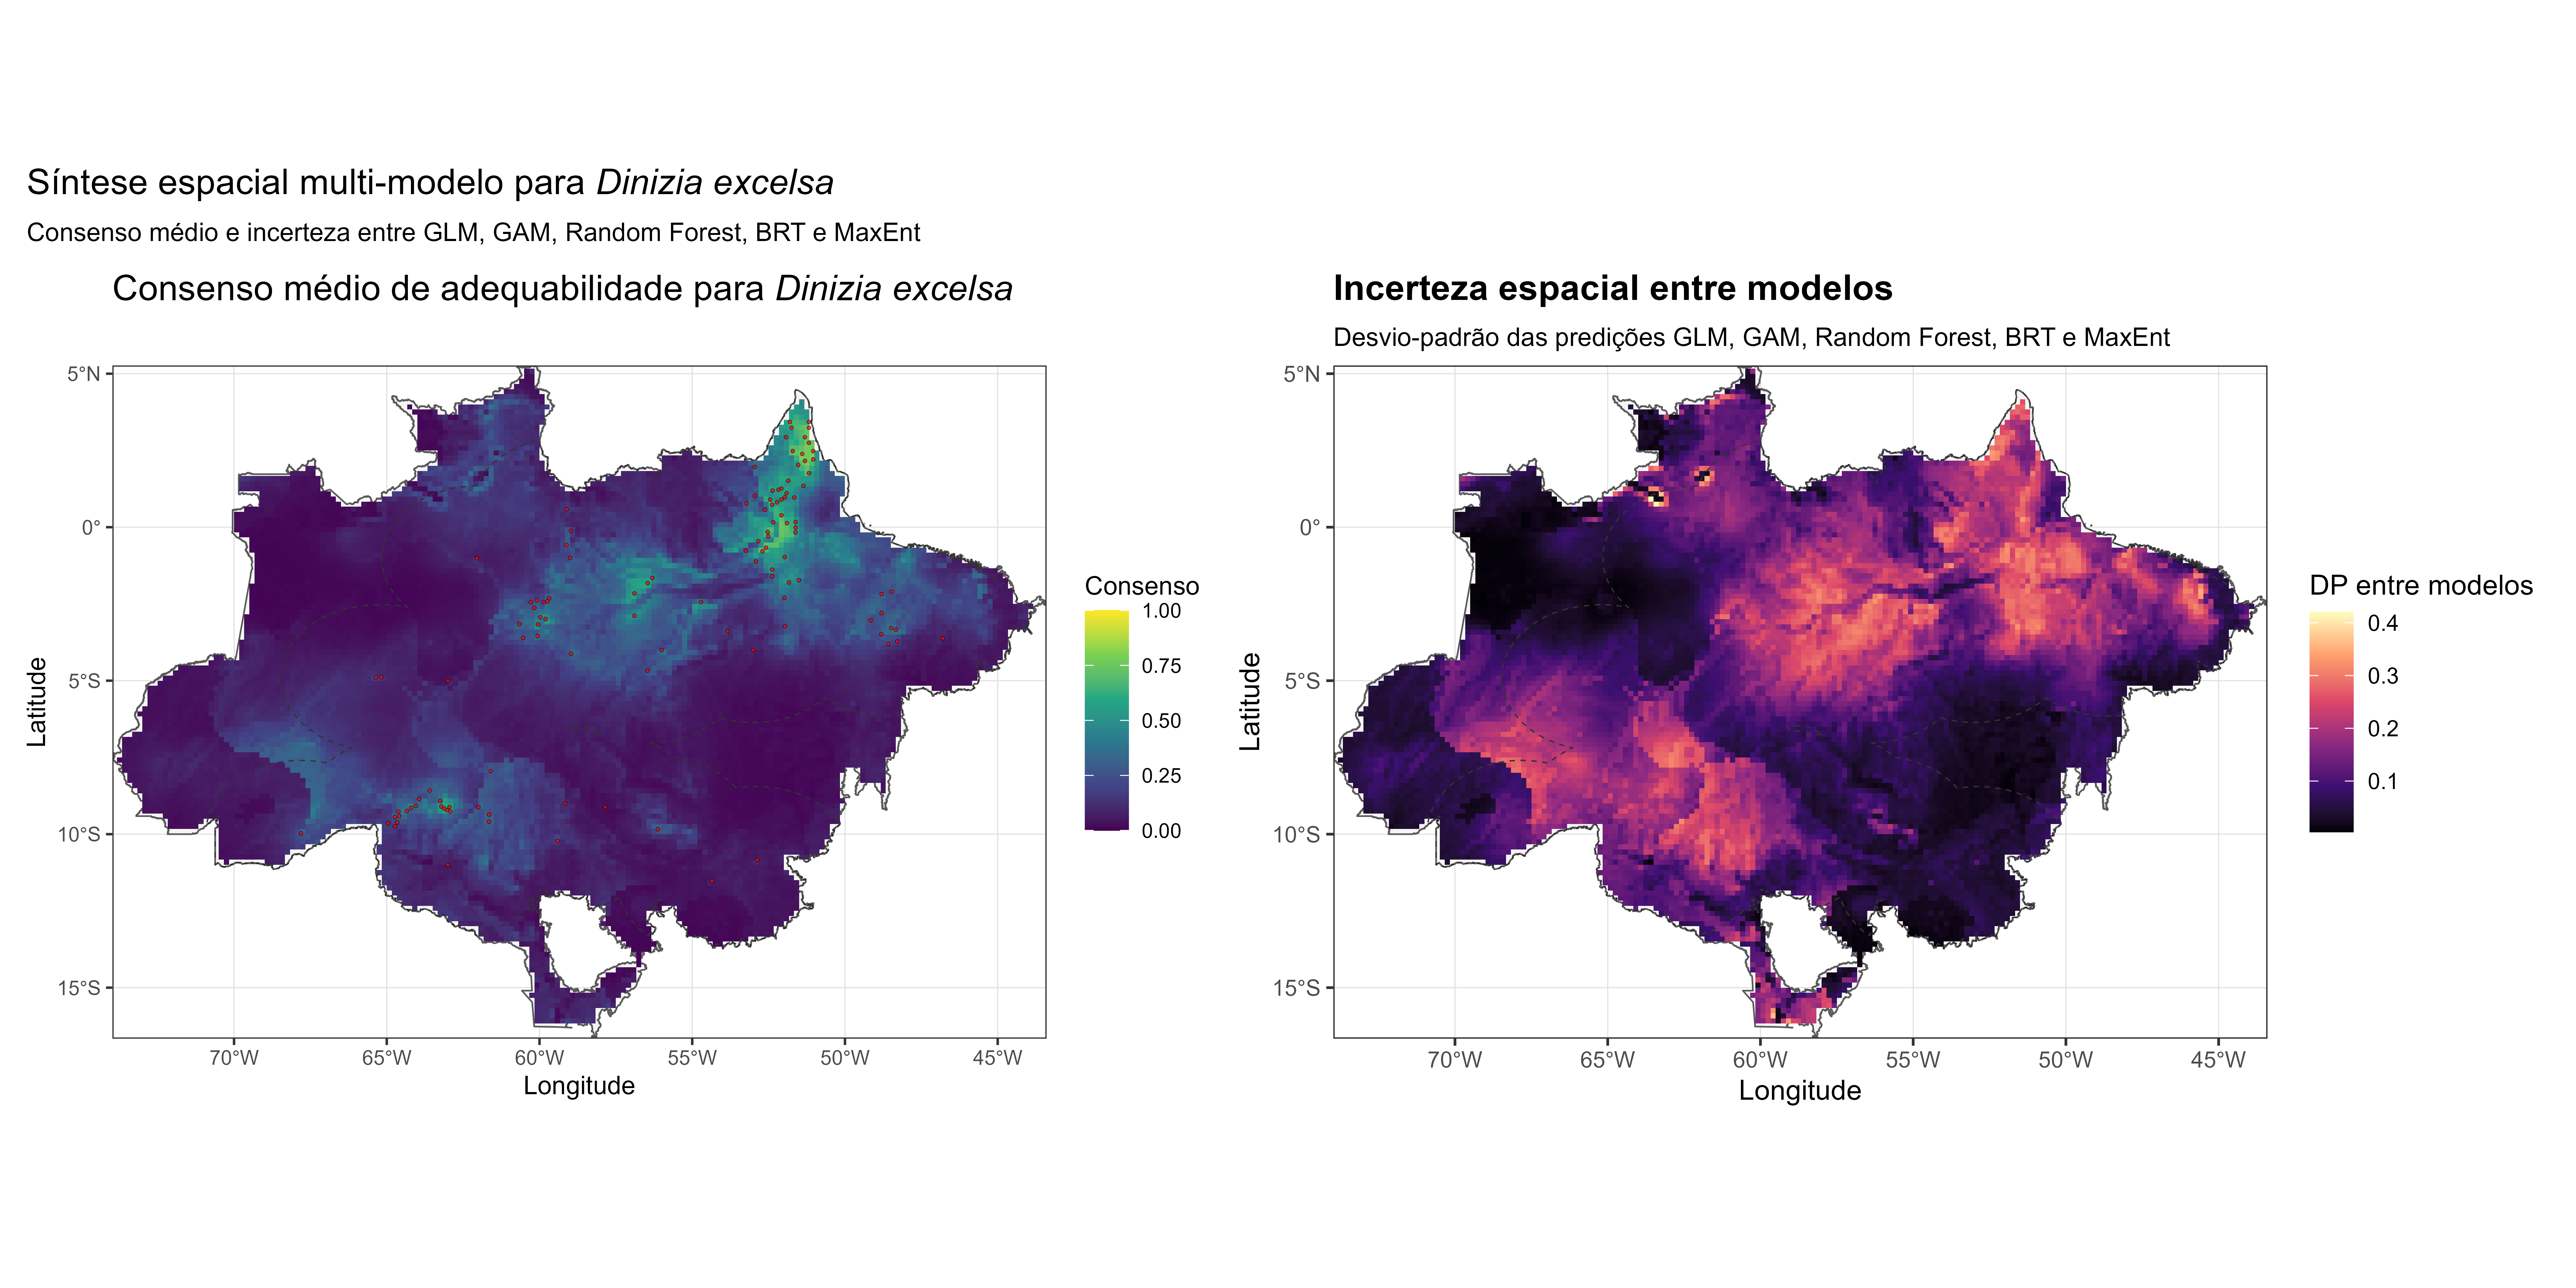
\includegraphics[width=\textwidth]{figuras/unidade10/unidade10_sintese_consenso_incerteza_glm_gam_rf_brt_maxent.png}
	\caption{
		Síntese espacial multi-modelo para \textit{Dinizia excelsa} no bioma Amazônia. 
		O painel esquerdo apresenta o consenso médio de adequabilidade ambiental obtido a partir da média das predições dos modelos GLM, GAM, Random Forest, BRT e MaxEnt. 
		O painel direito apresenta a incerteza espacial associada às predições, estimada pelo desvio-padrão entre os modelos. 
		Áreas com elevados valores de consenso indicam maior concordância quanto à adequabilidade ambiental da espécie, enquanto áreas com maior desvio-padrão representam regiões de maior divergência entre algoritmos e, consequentemente, maior incerteza preditiva.
	}
	\label{fig:unidade10_consenso_incerteza}
\end{figure}

\begin{conceito}[title={\faBook\quad Mensagem central}]
	Maxent não deve ser usado como uma caixa-preta. O desempenho do modelo depende da definição adequada da área acessível, da escolha do background, da seleção de variáveis, da regularização e da avaliação independente.
\end{conceito}

%=========================================================
\subsection*{Síntese comparativa dos algoritmos}

Após a apresentação dos principais algoritmos utilizados em SDM, torna-se
importante compreender suas diferenças conceituais, vantagens operacionais,
limitações metodológicas e potencial de interpretação ecológica. A
Tabela~\ref{tab:comparacao_algoritmos_sdm} apresenta uma visão integrada dos
métodos abordados nesta apostila, auxiliando na seleção do algoritmo mais
adequado para diferentes objetivos ecológicos e biogeográficos.

\begin{table}[H]
	\centering
	\caption{Comparação dos principais algoritmos utilizados em Modelagem de Distribuição de Espécies (SDM).}
	\label{tab:comparacao_algoritmos_sdm}
	
	\scriptsize
	
	\begin{tabular}{
			p{0.12\textwidth}
			p{0.16\textwidth}
			p{0.14\textwidth}
			p{0.21\textwidth}
			p{0.22\textwidth}
			p{0.11\textwidth}
		}
		
		\toprule
		\textbf{Método} &
		\textbf{Tipo de dado} &
		\textbf{Relação ecológica} &
		\textbf{Vantagens} &
		\textbf{Limitações} &
		\textbf{Interpretação} \\
		\midrule
		
		GLM &
		Presença--Ausência &
		Linear &
		Simples, robusto e amplamente utilizado &
		Baixa flexibilidade para relações complexas &
		Excelente \\
		
		GAM &
		Presença--Ausência &
		Não linear &
		Flexível e interpretável &
		Mais complexo que o GLM &
		Muito alta \\
		
		Random Forest &
		Presença--Ausência &
		Não linear &
		Elevado desempenho preditivo &
		Menor interpretabilidade ecológica &
		Média \\
		
		BRT &
		Presença--Ausência &
		Não linear &
		Captura interações e relações não lineares &
		Ajuste de hiperparâmetros delicado &
		Média \\
		
		Maxent &
		Presença--Background &
		Não linear &
		Excelente para dados de presença apenas &
		Sensível ao background e ao viés amostral &
		Boa \\
		
		Ensemble &
		Múltiplos &
		Integrado &
		Reduz a incerteza algorítmica &
		Maior complexidade de interpretação &
		Variável \\
		
		\bottomrule
		
	\end{tabular}
	
\end{table}

%=========================================================
\subsection*{Guia prático de seleção de algoritmos}

\begin{table}[H]
	\centering
	\caption{Guia prático para seleção de algoritmos em diferentes aplicações de SDM.}
	\label{tab:guia_escolha_algoritmos}
	
	\small
	
	\begin{tabular}{
			p{0.48\textwidth}
			p{0.36\textwidth}
		}
		
		\toprule
		\textbf{Situação} &
		\textbf{Método recomendado} \\
		\midrule
		
		Poucos registros de ocorrência &
		Maxent \\
		
		Interpretação ecológica dos efeitos ambientais &
		GLM ou GAM \\
		
		Predição com máximo desempenho estatístico &
		Random Forest ou BRT \\
		
		Modelagem para conservação da biodiversidade &
		Ensemble \\
		
		Projeções sob mudanças climáticas &
		Ensemble \\
		
		Análise exploratória inicial &
		GLM \\
		
		Curvas de resposta ecológica &
		GAM \\
		
		Avaliação da importância relativa das variáveis &
		Random Forest ou BRT \\
		
		Dados de presença apenas &
		Maxent \\
		
		Redução da incerteza algorítmica &
		Ensemble \\
		
		\bottomrule
		
	\end{tabular}
	
\end{table}

%=========================================================
\begin{center}
	\fbox{
		\begin{minipage}{0.90\textwidth}
			
			\textbf{Síntese metodológica.}
			
			Não existe um algoritmo universalmente superior para todos os problemas
			ecológicos. O desempenho de um modelo depende da qualidade dos dados,
			da definição da área acessível ($M$), da seleção de variáveis ambientais,
			da estratégia de validação e da pergunta ecológica proposta.
			
			Em aplicações modernas de conservação e mudanças climáticas, abordagens
			\textit{ensemble} são frequentemente recomendadas por reduzirem a dependência
			de algoritmos individuais e fornecerem estimativas mais robustas da
			adequabilidade ambiental.
			
		\end{minipage}
	}
\end{center}
%=========================================================

\section{Exercícios de fixação}

\begin{enumerate}
	\item Explique o princípio da máxima entropia.
	\item Diferencie dados de presença, ausência e background.
	\item O que são feature classes no Maxent?
	\item Qual o papel da regularização?
	\item Por que modelos Maxent muito complexos podem ser problemáticos?
	\item Explique por que tuning é necessário em Maxent.
	\item Compare Maxent com GLM, GAM, Random Forest e BRT.
\end{enumerate}

% ============================================================
% UNIDADE 11
% ============================================================

